\chapter[Introducción]{Introducción}
\label{ch:intro}

\section{Motivación}
\label{sec:motivacion}
Con los actuales avances tecnológicos, el reconocimiento de expresiones faciales (FER, Facial Expression Recognition) forma parte importante de una rama de la inteligencia artificial, específicamente el reconocimiento de patrones.  Las investigaciones sobre el FER permiten el desarrollo de futuras tecnologías ligadas al desarrollo de interfaces centradas en el humano. 

Existen diversas aplicaciones tecnológicas enfocadas al reconocimiento de expresiones faciales aplicadas en distintas áreas del conocimiento humano, tales como:  la medicina, que se utiliza para la detección de enfermedades y rehabilitación de trastornos mentales; la psicología, para reportes sobre estados de ánimo; el marketing, la posibilidad de una segmentación del cliente al cual se quiere llegar con la publicidad; la robótica, la interacción humano-robot; la seguridad, para combatir fraudes de pasaportes, soporte al orden público e identificación de personas desaparecidas; entre otras áreas.

Diversas empresas también han utilizado estos avances de reconocimiento facial como un componente que aporta información en las tecnologías que ofrecen. Un ejemplo de esto es  Google que utiliza el FER en su motor de búsqueda de imágenes y se proyecta utilizar este reconocimiento para aportar información a la entrada de video de los Google Glass~\cite{GoogleGlass}. Otro ejemplo es Facebook que usa la detección de rostros en  fotos para realizar el etiquetado rápido de usuarios.

Los estudios de Mehrabian~\cite{Mehrabian1968} sobre la comunicación oral indican que las expresiones faciales contribuyen con aproximadamente el 55\% de la transmisión del mensaje, lo cual es un valor mucho mayor que la parte verbal con 7\% y la parte vocal un 38\%.

El objetivo de este proyecto es buscar un nuevo descriptor espacio temporal para reconocer expresiones faciales. Para esto se propone un nuevo método utilizando imágenes dinámicas, el cual utilizaremos para reconocer las seis expresiones faciales universales: alegría, asco, ira, miedo, sorpresa y tristeza.

\section{Problema}
\label{sec:problema}

En la actualidad existen muchos métodos que permiten resolver el problema del reconocimiento de expresiones faciales, algunos utilizan el sistema de codificación de acciones faciales (FACS) creado por Ekman~y~Friesen~\cite{Ekman1978}, entre los cuales están las investigaciones de Pantic y Rothkrantz~\cite{Pantic2004}, Lien et al.~\cite{Lien1998}, Pantic y Patras~\cite{Pantic2006}, entre otros. Otras investigaciones utilizan métodos de reconocimiento basados en características geométricas o de apariencia, entre los cuales están Ramírez et al.~\cite{RamirezRivera2013}, utilizando Local Direccional Number Patterns; Lyons et al.~\cite{Lyons1998}, utilizando filtros de Gabor; Ahonen et al.~\cite{Ahonen2006}, utilizando Local Binary Patterns (LBP por sus siglas en inglés).

Las últimas investigaciones se centran en poder resolver el problema del reconocimiento de expresiones agregando la variable temporal $t$, la cual indica que ya no solo se quiere reconocer en imágenes sino que en secuencias de imágenes o videos, con lo cual además de necesitar crear algoritmos que permitan buscar la expresión a través del tiempo, también deben ser algoritmos eficientes, debido a la gran cantidad de cálculos que se deben realizar. Existen distintas investigaciones que intentan resolver el problema del reconocimiento en vídeos: Zhao y Pietikäinen~\cite{Zhao2006}, crean una nueva codificación basada en LBP introduciendo la variable del tiempo, esta codificación recibe el nombre de Volume Local Binary Patterns; Zhao y Pietikäinen~\cite{Zhao2006}, también crean otra codificación basada en LBP en la cual utilizan tres planos ortogonales, llamada LBP-TOP; Buenaposada~\etal~\cite{Buenaposada2008}, estiman la deformación de los componentes no rígidos del rostro; Yeasin~\etal~\cite{Yeasin2004}, crean una firma temporal de cada entrada, con la cual entrenan sus modelos; Xiang~\etal~\cite{Xiang2008}, utilizan la transformada de Fourier para realizar la extracción de características, y luego utilizan Fuzzy C-means para generar los modelos.

En este trabajo proponemos un nuevo método que nos permita poder resolver el problema del reconocimiento de expresiones faciales en videos. La idea general de nuestra solución es juntar métodos de distintas áreas de las ciencias de la computación y crear una nueva forma de representar las expresiones faciales en video. En general introducimos un nuevo micro-descriptor que llamamos \textit{rayo de flujo}, el cual junto con técnicas de aprendizaje maquina (machine learning, en inglés), recuperación de información (information retrieval, en inglés), visión por computador (computer vision, en inglés) y reconocimiento de patrones (pattern recognition, en inglés), nos permitirán crear un modelo que realice el reconocimiento de las seis expresiones faciales universales. 

 %ésta debe ser una solución robusta, puesto que es necesario poder lograr resultados comparables con los actuales métodos ya creados. Esta solución debe poder responder preguntas como ¿Es posible crear un modelo de clasificación a partir de las teorías propuestas en este trabajo?, de ser así, ¿Qué tan buena es la representación creada por el modelo?, ¿Cómo se compara con los algoritmos que ya resuelven este problema?, ¿Qué tan eficiente es con respecto al tiempo de ejecución es el algoritmo?, ¿Es posible implementar esta idea para reconocimiento en tiempo real?, \etc.



\section{Solución propuesta}
\label{sec:solucion}

Para este nuevo método se introduce un nuevo micro-descriptor, el cual nos permite realizar el seguimiento de las regiones de interés (ROI, regions of interest) que denominaremos \textit{rayo de flujo} o simplemente \textit{rayo}.


\subsection{Pipeline}

La cadena de procedimientos ordenados o \textit{pipeline} de este método se divide en cuatro grandes etapas: preprocesamiento de la base de datos, extracción de micro-descriptores, creación de macro-descriptores, y entrenamiento y clasificación, este procedimiento puede ser visto en la Figura~\ref{intro:fig:pipeline}.
	\begin{figure}[b]
		\centering
		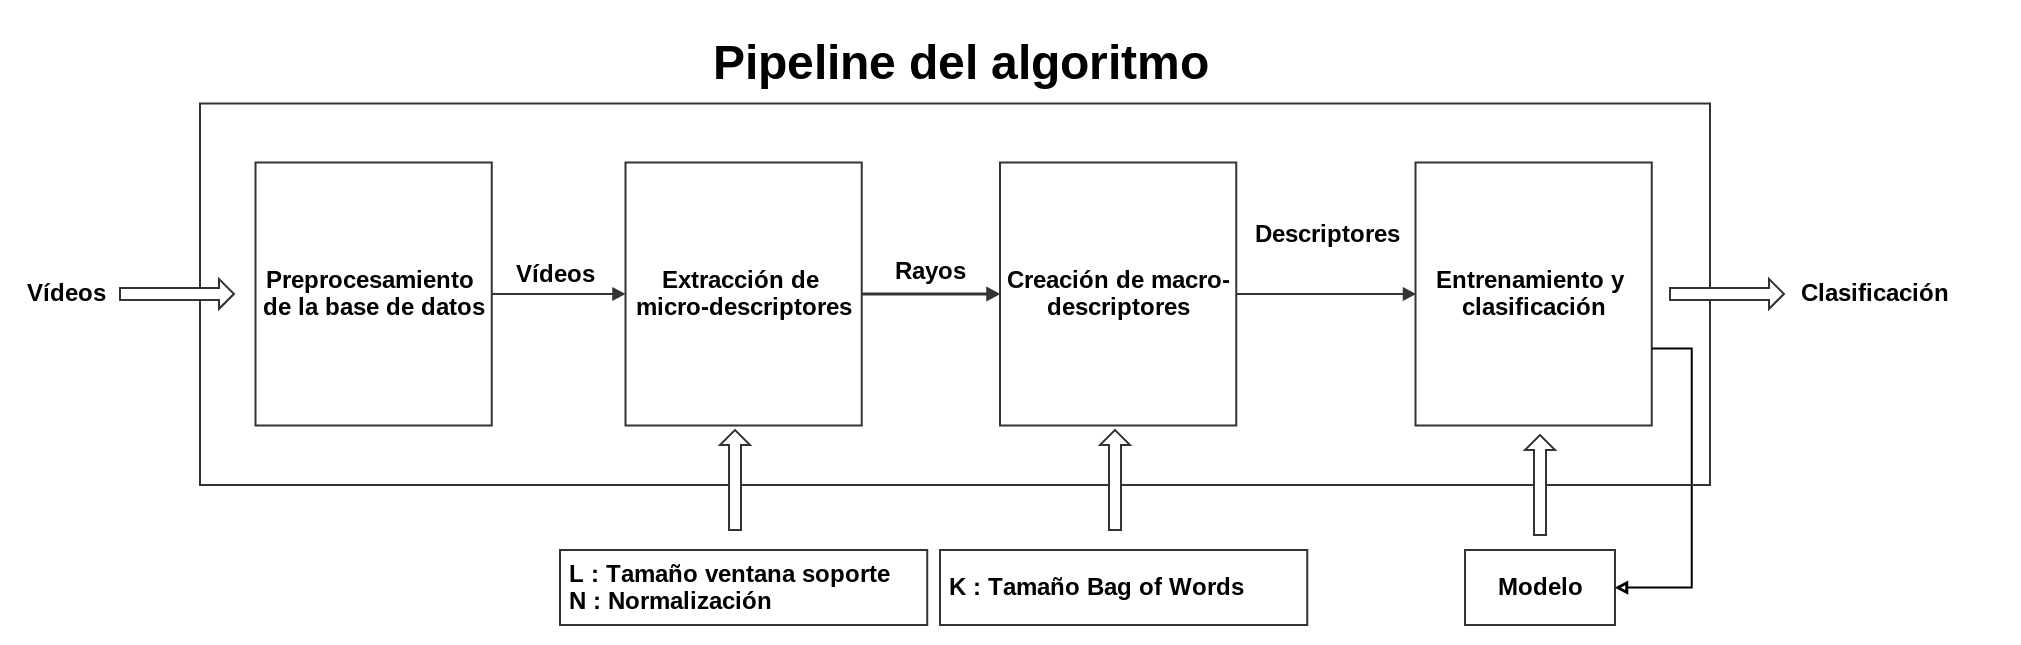
\includegraphics[width=1\textwidth]{Figuras/Diagramas/pipeline.png}
		\caption{Pipeline del algoritmo propuesto.}
		\label{intro:fig:pipeline}
	\end{figure}		
	
\textbf{Preprocesamiento de la base de datos.}
Antes de poder realizar la extracción de características de los videos, es necesario realizar un preprocesamiento sobre éstos, esto debido a que los videos pueden tener ciertos elementos que estropean la extracción de características. Para evitar agregar ruido al video se utilizan dos técnicas que permiten obtener solo el rostro de la persona a representar su expresión y a su vez corregir los movimientos que éstos puedan tener. Esta etapa será profundizada en la Sección~\ref{sec:proc_bdd}.


\textbf{Extracción de micro-descriptores.}
Este proceso consiste en la extracción de los rayos de flujo de cada uno de los videos preprocesados, para esto, primero se seleccionan las regiones de interés de la cara. Luego, para cada uno de los pixeles de la región, se procede a calcular el movimiento de este píxel con respecto al cuadro siguiente, y así sucesivamente con cada uno de los cuadros del vídeo. Luego de calcular el movimiento para cada píxel en cada cuadro, se obtiene el conjunto de \textit{rayos} o micro-descriptores que definen el video. Esta etapa será profundizada en la Sección~\ref{sec:micro_descriptores}.


\textbf{Creación de macro-descriptores.}
Luego de extraer cada uno de los micro-descriptores, se procede a crear utilizar la técnica de la bolsa de palabras visuales (\textit{Bag of Visual Words} en inglés), este método es utilizado para poder agrupar los \textit{rayos} en $k$ grupos, los cuales definen el espacio de los macro-descriptores. Cada \textit{rayo} extraído de los vídeos pertenece únicamente a un solo grupo, por lo tanto es posible para cada vídeo obtener un histograma de la frecuencia de aparición de cada uno de estos grupos en sus \textit{rayos}. Este histograma obtenido es el macro-descriptor que se utiliza para poder entrenar y clasificar. Esta etapa será profundizada en la Sección~\ref{sec:macro-descriptores}.


\textbf{Entrenamiento y clasificación.}
Luego de obtener los macro-des\-crip\-tores para cada uno de los vídeos, se procede a la etapa de entrenamiento y posterior clasificación. Para poder entrenar y clasificar con los macro-descriptores obtenidos en la etapa anterior, se utilizan las Maquinas de Vectores de Soporte (Support Vector Machines por sus siglas en ingles). Esta técnica permite dividir el espacio vectorial representado por los descriptores de entrenamiento, para luego ser probado por los descriptores que se obtienen en la clasificación o prueba del modelo creado. Para poder probar la efectividad de la clasificación se utiliza la técnica de validación cruzada, la cual permite realizar distintas pruebas de entrenamiento y clasificación, para obtener cual es el porcentaje de efectividad del método. Esta etapa será profundizada en la Sección~\ref{sec:clasificacion}.

\subsection{Ventajas potenciales del método}
\label{intro:ventajas}
En esta investigación se introduce un nuevo micro-descriptor llamado \textit{Rayo de flujo}, en simples palabras, 
un \textit{rayo de flujo} es el conjunto de variaciones que tiene un píxel determinado a lo largo del vídeo, esto será explicado en mayor profundidad en la Sección~\ref{sec:micro_descriptores}.

Éste, al ser un enfoque nuevo no visto en otras investigaciones, las distintas ventajas potenciales serán evaluadas a lo largo de la investigación, en general nos centraremos en demostrar o desmentir las siguientes incógnitas:

\begin{itemize}
	\item ¿Permitirán los \textit{rayos} realizar un modelado espacio-temporal?
	\item Al ser un modelado espacio-temporal de los píxeles, los \textit{rayos}, ¿permitirán ver cual es el comportamiento de los pixeles a través del tiempo?
	\item ¿Permitirán los \textit{rayos} modelar micro-patrones en los movimientos del rostro que no pueden ser vistos a simple vista por los humanos?, de ser cierto, ¿estos micro-patrones aportarán mayor información al modelo de clasificación?.
	\item ¿Existe la posibilidad de que cada una de las expresiones faciales universales pueda tener asociado un conjunto de \textit{rayos} que la definan?. 
\end{itemize}


\section{Objetivos}
\label{subsec:objetivos}
A continuación se describen los objetivos de este trabajo:

\subsection{Objetivo general}
\label{subsubsec:objgeneral}
Crear un descriptor espacio-temporal basado en el seguimiento del movimiento de los pixeles para el reconocimiento de expresiones faciales en video.

%Crear un descriptor para el reconocimiento de expresiones faciales en vídeo utilizando micro patrones basados en el seguimiento del flujo de los movimientos del rostro.
%\item Crear o encontrar una métrica que permita la comparación entre rayos luego del proceso de normalización.
%\item Evaluar y comparar el método creado con el estado del arte hasta antes de comenzar la memoria. 
%\item Definir un método de elección de las regiones de interés del rostro.
%\item Definir un método de elección de las regiones de interés del rostro.

\subsection{Objetivos específicos}
\label{subsubsec:objgeneral}
	\begin{enumerate}
		\item Modelar el comportamiento de los pixeles a través del tiempo.
		\item Definir una codificación que permita la normalización de los rayos de flujo.
		\item Estudiar la distribución de los movimientos de los pixeles sobre el rostro.
	\end{enumerate}